% dependencies: xelatex, xecjk package,wenquanyi中文字体,也可以设置其他的中英文字体
%!TEX program = xelatex
\documentclass[11pt]{article}
\usepackage[boldfont]{xeCJK}
\usepackage{amsfonts}
\usepackage{amsmath}
\usepackage{hyperref}
\usepackage{esvect} %一个更好的矢量描述工具
%\setmainfont{Courier New} % 设置英文衬线字体
% \setmonofont{} % 设置英文等宽字体,等宽英文字体大全:http://zh.wikipedia.org/wiki/%E7%AD%89%E5%AE%BD%E5%AD%97%E4%BD%93
% \setsansfont{} % 设置英文无衬线字体
\setCJKmainfont{WenQuanYi Micro Hei} % 设置缺省中文字体
%\setCJKfamilyfont{WenQuanYi Micro Hei} % 与setCJKmainfon t等同,http://bbs.ctex.org/forum.php?mod=viewthread&tid=51057
\parindent 2em   %段首缩进
 
\begin{document}
%%%%%%%%%%%%%%%%%%%%%%%%%%%%%%%%%%%%%%%%%%%%
%    这里是文档的开头                                                                                                                      %
%%%%%%%%%%%%%%%%%%%%%%%%%%%%%%%%%%%%%%%%%%%%
\title{多旋翼飞行器动力学建模中的数学知识}
\author{杨硕}

\maketitle
这篇教程围绕多旋翼飞行器的动力学模型展开介绍,对旋转表示法、角速度、惯量、欧拉角、四元数、欧拉方程等概念进行深入讲解。

一般来说,研究多旋翼飞行器的工程师和科学家们都是电子、机械、计算机科学背景,他们除了非常基本的数学物理课程之外,可能并没有系统地学习基本的经典力学知识和代数知识。
然而按照正统的数学和物理课程学习相关知识又会花费过多的时间,因此我认为通过多旋翼飞行器控制中对数学要求最高的部分:动力学建模,穿插介绍相关的数学物理知识,是一个比较方便整理思路并且易于理解的学习方法。
因为每一个数学或者物理的知识点被介绍出来之后,都会立即应用到实际的工程问题中,读者很直观地看到如何用数学和物理知识指导实际需求。

本教程尽量用明白清晰的语言介绍各个知识点,同时尽量不跳过任何公式推导的中间过程。有些地方可能会显得行文冗长多余,数学功底好的读者可以略去公式前后文的解释。

\section{基本符号定义和坐标系定义}
本节介绍一些基本的符号定义以及飞行器控制中常用的坐标系定义,教程剩余章节中将大量使用本节中的符号。
\subsection{基本符号定义}
$a$,小写字母表示标量,或者作为名字指代某一概念,比如坐标系的$x$轴

$\vv{v}$,字母上加箭头表示矢量。很多教材会使用黑体字母,如$\bf{v}$,来表示矢量,这样一方面容易和矩阵混淆,一方面容易和标量混淆。虽然箭头在有些公式中显得过于复杂,但是能够方便地让读者时刻记得公式中符号的数学意义。

$\dot{a}$,代表对标量求导,我们默认标量$a$是以$t$为自变量的函数$a(t)$,因此就把$t$隐去以简化符号。

$\dot{\vv{v}}$或$\frac{d\vv{v}}{dt}$,代表对矢量求导,我们默认矢量$\vv{v}$中每一个元素$v_i$都是以$t$为自变量的标量函数

$\bf{A}$,黑体大写字母表示矩阵

$\bf{I}_{3x3}$,有时会通过下标的方式指明矩阵的尺寸。常见的例子是用来指明单位矩阵(Identity Matrix)$\bf{I}$的尺寸,比如3乘3的单位矩阵表示为$\bf{I}_{3x3}$。

$\bf{A}^{-1}$,对矩阵求逆

$\bf{A}^T$,对矩阵求转秩

$\bar{\bf{q}}$,表示四元数

${\bf R}_{ab}$,表示旋转矩阵,$a$和$b$代表两个\textbf{原点相交}的坐标系,旋转矩阵将$b$坐标系中表示的矢量旋转到$a$坐标系中

$\bar{\bf{q}}_{ab}$,表示旋转四元数,下标的含义与旋转矩阵中的定义相同。

$\lfloor \vv{\omega} \ \times \rfloor$,将矢量$\vv{\omega}$变换成反对称矩阵$\lfloor \vv{\omega} \ \times \rfloor$(将会在后面详细介绍)

其他未说明的符号一部分是标准的数学计算符号,另一部分则在教程中定义
\subsection{坐标系定义}
航空航天工程中发展出了描述飞行器在空间中相对于地球的标准表达方式。在描述动力学模型中,我们只需要关心大地坐标系和机体坐标系。
\subsubsection{大地坐标系}
飞行器放置在地面上,启动之后飞行器离开这一地点,但是很多的传感器都是以地面上这一点作为基准点的。为了描述飞行器相对于这一地面基准点的位置和姿态角,我们要在地面上附加一个坐标系,叫做大地坐标系(ground frame)或者地球坐标系(earth frame)。相应地,有时也会将这种坐标系缩写为坐标系$g$或者坐标系$e$。本教程中我们用$e$来指代大地坐标系,$e$会出现在很多公式符号的下标中,特别是旋转矩阵和旋转四元数的下标中。

\begin{center}
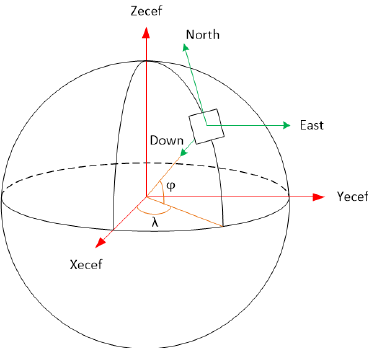
\includegraphics[width=0.6\textwidth]{images/ned.png}
\end{center}

大地坐标系遵循一般笛卡尔坐标系中坐标轴关系,三个坐标轴的指向与地理方位相关。在基准点上,$x$轴指向北方,$y$轴指向东方,$z$轴指向地心。因此,大地坐标系也被称作“北东地”坐标系(NEG frame)。
\subsubsection{机体坐标系}\label{sec:bodyframe}
飞行器上也需要附加一个坐标系,以便描述飞行器自身的部件位置,以及描述自身的旋转。无论飞行器如何变换自身的姿态,这个坐标系相对于飞行器的位置不会发生变化。机体坐标系的坐标轴关系与一般笛卡尔坐标系相同,某些情况下还有可能和大地坐标系重合(在飞行器准备起飞的时候,我们通常把机体坐标系和大地坐标系设定重合起来),只是我们将$x$轴称为“横滚”轴(roll axis)、$y$轴称为“俯仰”轴(pitch axis)、$z$轴称为“偏航”轴(yaw axis)。如下图所示:
\begin{center}
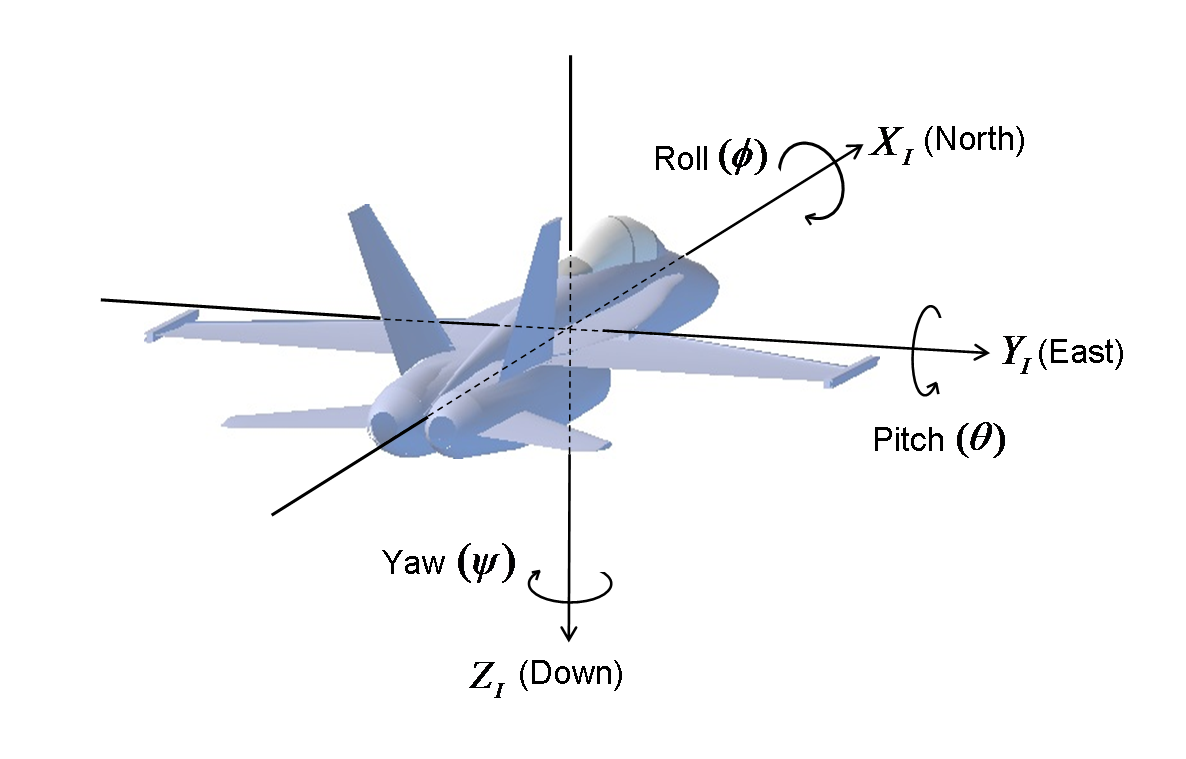
\includegraphics[width=0.8\textwidth]{images/InertialFrame.png}
\end{center}

本教程中我们用$b$来指代机体坐标系。

\section{旋转矩阵}\label{sec:rotmtx}
在定义坐标系之后,我们所关注的问题是如何描述飞行器相对地面的位置和姿态。对位置来说,如果把飞行器看做质点,那么我们可以很容易地在大地坐标系中描述出飞行器的三维位置,这个位置通常用$\vv{p}$来表示:
$$
\vv{p} = p_1\vv{i}+p_2\vv{j}+p_3\vv{k}
$$
其中$\vv{i}$,$\vv{j}$,$\vv{k}$分别是坐标系$xyz$三轴的单位向量:
$$
\vv{i} = \begin{bmatrix}
1\\0\\0
\end{bmatrix}\ \ \ \ \ 
\vv{j} = \begin{bmatrix}
0\\1\\0
\end{bmatrix}\ \ \ \ \ 
\vv{k} = \begin{bmatrix}
0\\0\\1
\end{bmatrix}
$$
这样我们也可以把单位向量合并起来,把$\vv{p}$简单写成$\vv{p} = \begin{bmatrix}
p_1\\p_2\\p_3
\end{bmatrix}$。在后面的教程中,我们会经常切换两种表示方法以便于解释不同的问题。

在实际中,飞行器并非一个质点,而是\textbf{无数个质点构成的刚体}。为了描述这个刚体相对于大地坐标系的姿态,我们需要引入旋转矩阵的概念。另外我们可以说“飞行器的某个电机位于飞行器质心一侧的30厘米处”,并且能够通过机体坐标系定量地描述电机位置与质心的关系。但是为了描述电机位置,或者说对于刚体上不位于质心的任意一点相对于大地坐标系原点的关系,必须要借助旋转矩阵来描述。
\subsection{通过旋转矩阵描述坐标系之间的旋转变换}\label{sec:rotationmtxdefinition}
这一节中我们暂时不用飞行器和大地坐标系的术语,而是考虑更一般的情况。

假设空间中有一个坐标系$e$(也可以用$OXYZ$来表示,因为我们用$\vv{OX}$、$\vv{OY}$、$\vv{OZ}$来称呼它的三个轴),有一个刚体处于这个坐标系中,我们在刚体上附加机体坐标系$b$(也可以用$oxyz$来表示,同理它的三个轴是$\vv{ox}$、$\vv{oy}$、$\vv{oz}$)。初始时坐标系$e$和坐标系$b$是重合的。假设刚体因为某些原因变换了姿态,那么坐标系$b$的各轴就不再与坐标系$e$的各轴重合,不过他们的原点依然是重合的。
%%%%%%%%%%%%%插个图
%%%%%%%%%%%%%
为了描述变换姿态后坐标系$b$和坐标系$e$之间的关系,我们注意到坐标系$b$的各轴在坐标系$b$中可以用前述的$\vv{i}$、$\vv{j}$和$\vv{k}$来表示,但是如果从坐标系$e$中观察,坐标系$b$的各轴就可以看做坐标系$e$中的普通矢量,那么坐标系$b$的一个轴可以表示成坐标系$e$的三个轴的线性组合。也即
$$
\vv{ox} = r_{11}\vv{OX} + r_{21}\vv{OY} + r_{31}\vv{OZ} 
$$
$$
\vv{oy} = r_{12}\vv{OX} + r_{22}\vv{OY} + r_{32}\vv{OZ} 
$$
$$
\vv{oz} = r_{13}\vv{OX} + r_{23}\vv{OY} + r_{33}\vv{OZ} 
$$
这里的$r_{ij}$表示线性组合的系数,我们可以不失一般性地就把他们当做9个常数。如果我们把这9个数字写成矩阵的形式(注意下标的顺序)
$$
{\bf R} = \begin{bmatrix}
r_{11} & r_{12} & r_{13}\\
r_{21} & r_{22} & r_{23}\\
r_{31} & r_{32} & r_{33}
\end{bmatrix}
$$
注意到$\vv{OX}$、$\vv{OY}$和$\vv{OZ}$其实是坐标系$e$中的$\vv{i}$、$\vv{j}$和$\vv{k}$,我们可以发现
$$
\vv{ox} = r_{11}\vv{OX} + r_{21}\vv{OY} + r_{31}\vv{OZ}  = 
\begin{bmatrix}
r_{11}\\
r_{21}\\
r_{31}
\end{bmatrix} =
\begin{bmatrix}
r_{11} & r_{12} & r_{13}\\
r_{21} & r_{22} & r_{23}\\
r_{31} & r_{32} & r_{33}
\end{bmatrix}
\begin{bmatrix}
1\\
0\\
0
\end{bmatrix} = {\bf R} \vv{i}
$$
同样地
$$
\vv{oy} =   {\bf R} \vv{j}
$$
$$
\vv{oz} =   {\bf R} \vv{k}
$$

在上述的推导中,我们需要注意一个细节:通常我们把任何笛卡尔坐标系的三个轴都称作$\vv{i}$、$\vv{j}$和$\vv{k}$。当我们谈论一个坐标系变换到另一个坐标系的问题时,问题中其实涉及了“$a$坐标系的$\vv{i}$、$\vv{j}$和$\vv{k}$”以及“$b$坐标系的$\vv{i}$、$\vv{j}$和$\vv{k}$”。更具体一点,在开始推导时,$\vv{OX}$是坐标系$e$的$\vv{i}$,而$\vv{ox}$是坐标系$b$的$\vv{i}$,但是后来获得$\vv{ox} =   {\bf R} \vv{i}$时,这里的$\vv{ox}$则是表达在坐标系$e$中。初看这会让人迷惑不解,但理解之后读者会发现这是比较不容易引起误解的描述方法。这样我们还可以将矩阵${\bf R}$写成
$$
{\bf R} = \begin{bmatrix}
\vv{ox} & \vv{oy} & \vv{oz}\\
\end{bmatrix}
$$

因此,假设现在刚体上有一点$\vv{p}$,它在坐标系$b$中是$\vv{i}$、$\vv{j}$和$\vv{k}$的线性组合,在坐标系$e$中则是$\vv{ox}$、$\vv{oy}$和$\vv{oz}$的线性组合,假设组合的系数是$p_1$、$p_2$和$p_3$。我们用$\vv{p_e}$代表点$\vv{p}$在坐标系$e$中的矢量形式,用$\vv{p_b}$代表点$\vv{p}$在坐标系$b$中的矢量形式,则
$$
\vv{p_e} = p_1\vv{ox}+p_2\vv{oy}+p_3\vv{oz}
$$
$$
\vv{p_b} = p_1\vv{i}+p_2\vv{j}+p_3\vv{k}
$$
显然地
$$
\vv{p_e} = {\bf R}\vv{p_b}
$$

我们说矩阵${\bf R}$将坐标系$b$中的点的表示转换到坐标系$e$中表示,它是一个\textbf{旋转矩阵}。这一物理含义可以用下标来描述,记为${\bf R}_{eb}$,所以最终我们写成
$$
\vv{p_e} = {\bf R}_{eb}\vv{p_b}
$$

另外根据矩阵的性质,我们还可以进行连续的旋转变换,比如
$$
\vv{p_e} = {\bf R}_{ea}{\bf R}_{ab}\vv{p_b}
$$
是将坐标系$b$中的点的表示变换到坐标系$a$,然后再变换到坐标系$e$。在后面介绍欧拉角的时候,我们会利用到连续变换的思想。

需要强调的是,$\vv{p_b}$和$\vv{p_e}$物理上都指代同一个质点,我们谈论的只是“表示”不同。就好比当我们谈论一下飞行器的高度时,它可以表示为“距离某幢楼楼顶10米”,也可以表示为“距离地面50米”。

\subsection{旋转矩阵的性质}\label{sec:rotationproperties}
上一节我们获得的
$$
{\bf R} = \begin{bmatrix}
\vv{ox} & \vv{oy} & \vv{oz}\\
\end{bmatrix}
= \begin{bmatrix}
r_{11} & r_{12} & r_{13}\\
r_{21} & r_{22} & r_{23}\\
r_{31} & r_{32} & r_{33}
\end{bmatrix}
$$
是非常一般性的结论,任意坐标系之间都有相同的变换关系。

因为$\vv{ox}$是坐标系$b$的$\vv{i}$,所以它是单位向量,而且与同为单位向量的$\vv{oy}$和$\vv{oz}$都正交。因此我们说${\bf R}$是一个单位正交矩阵(orthonormal matrix)。

通过基本线性代数之后和涉及叉乘的变换,我们可以证明以下两个性质
$$
{\bf R}^T{\bf R} = {\bf R}{\bf R}^T = \bf{I}
$$
$$
\text{det}(R) = 1
$$

事实上,这两个性质是${\bf R}$能够被称为笛卡尔坐标系之间变换的旋转矩阵的充要条件。所有这种旋转矩阵可以构成一个名为$SO(3)$的集合。$SO(3)$具有丰富的代数性质,本教程中不再详细讨论了。
%%%%%%%%%%%%%%%%%%%%%%%%%%%%%%%%%%%%%%%%%%
%%%                                           有时间还可以再写                                  %%%%%%%%%
%%%%%%%%%%%%%%%%%%%%%%%%%%%%%%%%%%%%%%%%%%

值得一提的时,上述推导全部是在三维笛卡尔坐标系中进行的,相似的推导也可以在二维笛卡尔坐标系中进行。读者可以自行推导,以加深对于旋转矩阵性质的理解。

\subsection{刚体变换}\label{sec:transform}
了解旋转矩阵之后,我们回到飞行器在大地坐标系中飞行的场景。现在我们可以通过一个辅助坐标系来描述飞行器上某个质点相对与大地坐标系原点的位置关系了。考虑下图中的场景:

我们用$OXYZ$来表示大地坐标系,$oxyz$来表示机体坐标系。然后我们建立中间坐标系$oXYZ$(注意大小写),由大地坐标系平移得到,所以中间坐标系$oXYZ$的各轴都与大地坐标系的各轴平行,而且中间坐标系$oXYZ$的原点与机体坐标系$oxyz$的原点重合。这样$OXYZ$和$oXYZ$之间仅有平移变换,而$oxyz$与$oXYZ$之间仅有旋转变换。
%%%%%%%%%%%%%插个图
%%%%%%%%%%%%%

假设原点$o$在大地坐标系$OXYZ$中的位置为$\vv{p}$,飞行器上某质点$\bf{q}$在机体坐标系$oxyz$中的位置为$\vv{r}$,$oxyz$与$oXYZ$之间的变换用旋转矩阵${\bf R}$表示,则很容易看出
\begin{equation}\label{eqn:transform}
\vv{q} = \vv{p} + {\bf R}\vv{r}
\end{equation}

公式右侧第二项中的符号为了公式整体的简洁简化了一些。如果再细致一些,我们可以定义“飞行器上某质点$\bf{q}$在机体坐标系$oxyz$中的位置的表示为$\vv{r}_b$,在中间坐标系$oXYZ$中的位置表示为$\vv{r}_e$,$oxyz$与$oXYZ$之间的变换用旋转矩阵${\bf R}_{eb}$表示”。这样我们有
$$
\vv{r}_e = {\bf R}_{eb}\vv{r}_b
$$
所以
$$
\vv{q} = \vv{p} + \vv{r}_e = \vv{p} + {\bf R}_{eb}\vv{r}_b
$$
我们可以进一步在这个公式中加入一些下标,以让他们所处的坐标系一目了然
\begin{equation}\label{eqn:transformsubs}
\vv{q}_{e} = \vv{p}_{eb} + {\bf R}_{eb}\vv{r}_b
\end{equation}
这里$\vv{p}_{eb}$指的是“坐标系$b$的原点在坐标系$e$中的位置”,整个公式意味着“质点在大地坐标系中的表示等于质点在机体坐标系中的表示乘以坐标系之间的旋转变换,再加上坐标系之间的平移变换”。读者应该用这一节的图例和公式\ref{eqn:transformsubs}理解“位置”、“表示”、“变换”之间的区别与联系。


\section{角速度}\label{sec:angular}
一个物体在空间中以恒定速度移动,同时进行了绕自身某个轴的旋转,这时物体上各点的速度各不相同。回想游乐园里的旋风旋转设施(spinning rides),站在大地上的观察者,会发现某些时刻能够看到转盘上自己的朋友相对静止,但是转盘另一侧的人则依然在高速旋转。理解角速度的原理能够帮助我们更好地理解运动的特性。

在章节\ref{sec:transform}中我们介绍了刚体变换,这一节中我们先从回顾高中物理中学过的角速度定义开始,推广到三维的情况,然后再把角速度和刚体变换连接起来。
\subsection{速度和角速度的关系-二维}	
%%%%%%%%%%%%%插个图
%%%%%%%%%%%%%
我们按图示建立二维笛卡尔坐标系,在二维平面上转动的点的位置可以用距离原点的距离$\vv{r}$和夹角$\theta$表示,角速度被定义为
$$
\omega = \frac{d\theta}{dt}
$$
根据微分的原理我们还知道点的速度大小是
$$
v = \frac{\|\vv{r}\|d\theta}{dt} = \omega \|\vv{r}\|
$$
花费一些篇幅介绍初等的二维的情况是想强调角速度“赝矢量”(pseudovector)的特性。中学物理中我们学过,即使是在最基本的二维情况下,$\omega$的方向也脱离了纸面:如果顺时针旋转,$\omega$的方向垂直纸面向内;如果逆时针旋转,$\omega$的方向垂直纸面向外。只有这样才能解释如何能够把方向互相垂直的$\vv{r}$、$\vv{v}$两个矢量通过$v = \omega \|\vv{r}\|$联系起来。虽然三者垂直让我们大约想到了叉乘的性质,但是这种解释有一种牵强附会的感觉。我们必须在三维场景中做更加仔细的推导。

\subsection{速度和角速度的关系-三维中的二维平面}	\label{sec:velandw}
考虑下图的三维笛卡尔坐标系,坐标系中有一质点在绕$z$轴逆时针转动。
%%%%%%%%%%%%%插个图
%%%%%%%%%%%%%

这个质点的轨迹处于一个垂直于$z$轴、平行于$xy$轴的平面上。按照上一节的定义,则质点的角速度的方向其实就是$z$轴,角速度用$\vv{\omega} = \frac{d\theta}{dt}\vv{k}$表示。我们用$\vv{r}_1$表示质点到$z$轴的距离,用$\vv{r}$表示质点到坐标系原点的距离。很显然地我们有
$$
\vv{v} = \vv{\omega} \times \vv{r}_1
$$
又因为$\vv{r}_1 = \vv{r} - \vv{r}_2$,而$\vv{r}_2$与$\vv{\omega}$重合,所以根据叉乘的性质
$$
\vv{v} = \vv{\omega} \times (\vv{r} - \vv{r}_2) = \vv{\omega} \times \vv{r} - \vv{\omega} \times \vv{r}_2 = \vv{\omega} \times \vv{r}
$$
\subsection{速度和角速度的关系-三维}\label{sec:velandangular3d}
接下来考虑一个更加一般的情况,以及另外一种表示方法下的推导方式。三维坐标系中的质点$\vv{r} = (x,y,z)$在绕$\vv{n}$所描述的轴转动,不失一般性地,我们可以把它的角速度写为
\begin{equation}\label{eqn:omegadef}
\vv{\omega} = \frac{d\theta}{dt}\vv{n} = \omega_1\vv{i}+\omega_2\vv{j}+\omega_3\vv{k}
\end{equation}

这种情况下的转动轴不垂直与坐标系的任何一个轴,这使得我们建立一个容易被描述的旋转所在的平面非常困难。这种情况下最好的办法是质点的运动投影到$xy$、$xz$和$yz$平面上分析每一个平面内的速度特性,然后再把每个平面上的分量叠加。这是物理学中常用的分析方法。
%%%%%%%%%%%%%插个图
%%%%%%%%%%%%%

首先先看$xy$平面,在这个平面中角速度的分量是$\omega_3\vv{k}$,质点投影的坐标是$P=(x,y)$,它距原点的距离为$r = \sqrt{x^2+y^2}$。我们考虑质点从$P$开始,在$\Delta t$时间内发生了一个微小的旋转,转过了$\Delta\theta = \omega_3\Delta t$,到达坐标$Q$,则矢量$\vv{PQ}$的长度为$|PQ| = r\Delta\theta$。如果把$Q$的坐标记为$(x+\Delta x, y + \Delta y)$,我们可以推导出
$$
\Delta x = - |PQ|\sin\theta = - r\Delta\theta \frac{y}{r} = -y \Delta\theta
$$
$$
\Delta y =  |PQ|\cos\theta =  r\Delta\theta \frac{x}{r} = x \Delta\theta
$$
则我们可以推出
$$
\text{在 $xy$平面中:} \frac{\Delta x}{\Delta t} = -y \omega_3 ,  \frac{\Delta y}{\Delta t} = x \omega_3
$$

在另外两个平面中做相似的推导,可以得到
$$
\text{在 $yz$平面中:} \frac{\Delta y}{\Delta t} = -z \omega_1 ,  \frac{\Delta z}{\Delta t} = y \omega_1
$$
$$
\text{在 $xz$平面中:} \frac{\Delta x}{\Delta t} = z \omega_2 ,  \frac{\Delta z}{\Delta t} = -x \omega_2
$$

现在我们再回到三维空间中。质点在三维空间的速度,实际上就是各个方向上位置变化的导数,可以写成
$$
\vv{v} = \frac{\Delta x}{\Delta t} \vv{i} + \frac{\Delta y}{\Delta t} \vv{j} + \frac{\Delta z}{\Delta t} \vv{k} =
\begin{bmatrix}
\frac{\Delta x}{\Delta t} \\
\frac{\Delta y}{\Delta t} \\
\frac{\Delta z}{\Delta t} 
\end{bmatrix}
$$
把之前推导的关系代入,则有
$$
\vv{v} = \begin{bmatrix}
\omega_2z - \omega_3y \\
\omega_3x - \omega_1z \\
\omega_1y - \omega_2x 
\end{bmatrix}
= \vv{\omega} \times \vv{r}
$$

上述三节中,我们用不同的方法推导出$\vv{v} = \vv{\omega} \times \vv{r}$,可见这是一个具有很强一般性的结论。它的物理意义是“质点对大地坐标系的速度等于绕某个轴旋转的角速度叉乘质点对大地坐标系的位置”。我们在后面的章节中还会见到更多的应用。

另外定义\ref{eqn:omegadef}中的表达式也呈现了角速度最一般的表示形式。在教程之后的章节中,我们会用$\vv{\omega} = [\omega_1\ \ \  \omega_2\ \ \  \omega_3]^T$来表示角速度。

\subsection{角速度传感器}\label{sec:angularsensor}
在刚体的运动中,角速度是一个非常关键的状态量。在多旋翼飞行器的控制中,我们必须能够测量这个状态量,才能对它施以准确有效的控制。然而准确测量角速度并不容易,几十年来,角速度传感器都是人类技术水平的一个标尺。目前比较成熟的角速度传感器有以下几种。
\subsubsection{机械陀螺}
旋转的刚体会呈现一种反直觉的物理特性:一个绕$z$轴高速旋转的刚体,如果在$x$轴上施加一个力矩,它会开始绕$y$轴缓慢旋转。在youtube上我们可以看到很多使用车轮实现演示的视频。在完善了欧拉方程的推导之后,我们会在章节\ref{sec:eulereqngyro}中简要介绍这一现象的物理原理。

\begin{center}
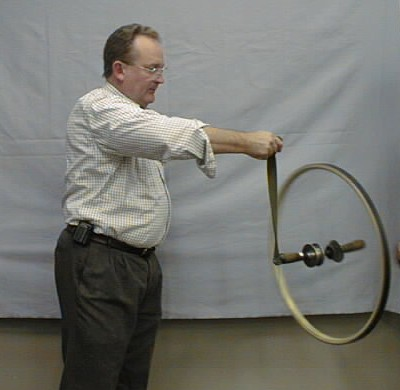
\includegraphics[width=0.6\textwidth]{images/BicycleWheelGyro.jpg}
\end{center}

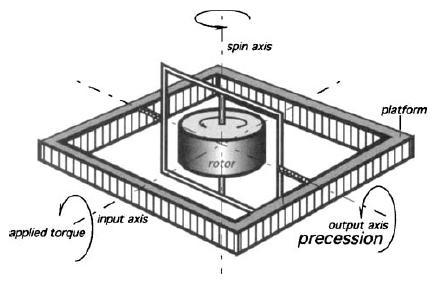
\includegraphics[width=0.8\textwidth]{images/gyroscopeAxes.jpg}

机械陀螺传感器利用了旋转刚体的这一特性,它的旋转刚体叫做陀螺。简单来说,如果按照上图中构成的传感器发生了绕input axis轴的转动,那么一定是因为input axis轴上有了外部施加的力矩。根据陀螺的output轴会发生的转动,我们可以进行反馈控制,给input axis轴施加一个反向力矩以消除陀螺的转动,施加的反向力矩等于外部施加的力矩,可以换算成角速度。

因为机械陀螺中有旋转的部件,并且涉及到反馈控制器,因此它的机械机构和软硬件系统都非常复杂。
\subsubsection{MEMS角速度传感器}
MEMS元器件是由大型集成电路的思想演变出来的新型机械制造工艺,在硅片上蚀刻、增加金属薄层,可以形成类似滑块、弹簧的结构。

\begin{center}
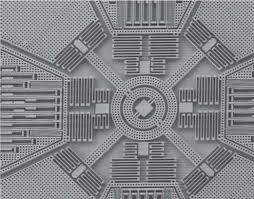
\includegraphics[width=0.6\textwidth]{images/memsgyro0.jpg}
\end{center}

如下图所示,MEMS角速度传感器包含一个或多个嵌在圆盘上的滑块,当传感器转动时,滑块会在向心力作用下发生移动,改变元器件整体的电容和电阻特性,因此能够用来检测向心力的大小,进而算出角速度的大小。

\begin{center}
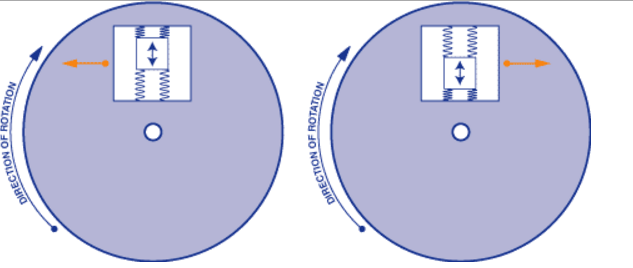
\includegraphics[width=0.6\textwidth]{images/memsgyro.png}
\end{center}
\subsubsection{光纤角速度传感器}
光纤角速度传感器利用了“赛格奈克效应”(Sagnac Effect),也即同一束光线分成两束分别穿过一个环形路线之后,整个环形路线的角速度就造成两束光线再汇合时出现相位差。这个原理在维基百科上有深入的讲解和推导。

\begin{center}
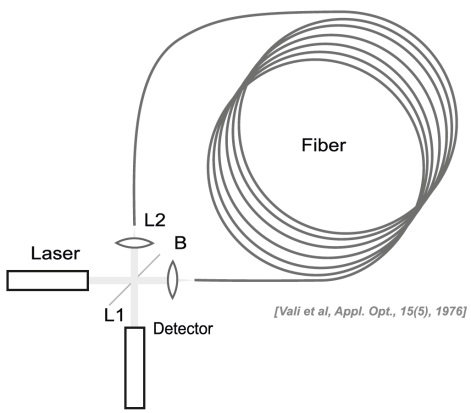
\includegraphics[width=0.6\textwidth]{images/sagnaceffect.jpg}
\end{center}

光纤角速度传感器中包含光源、相位检测装置和光纤构成的线圈。将这些元件整合入小尺寸的传感器中比较昂贵,另外一个光纤线圈只能测量一个轴的角速度,因此需要三套线圈才能测量三轴的角速度。但是光纤角速度传感器精确度较高、没有机械部件所以寿命长,相比前述两种传感器有比较大的优势,在军事设备上应用较多。

\ \\
\ \\
\ \\

很多资料中把角速度传感器都叫做“陀螺仪”,这种说法并不准确,因为除了机械陀螺仪中有旋转的陀螺以外,MEMS角速度传感器和光纤角速度传感器当中都不存在旋转的部件。

\subsection{角速度和旋转矩阵的关系}
我们回到公式\ref{eqn:transformsubs}
$$
\vv{q}_{e} = \vv{p}_{eb} + {\bf R}_{eb}\vv{r}_b
$$
在实际的运动中,我们应该把各个变化的量都看做关于时间的函数
\begin{equation}\label{eqn:transformt}
\vv{q}_{e}(t) = \vv{p}_{eb}(t) + {\bf R}_{eb}(t)\vv{r}_b
\end{equation}
注意到我们并没有把$\vv{r}_b$当做关于时间的函数。结合$\vv{r}b$的物理意义来看,这是一个合理的假设,因为通常来说飞行器的电机不会在空中相对质心发生移动。

对公式\ref{eqn:transformt}两边求导,我们可以获得
\begin{equation*}
\dot{\vv{q}}_{e}(t) =\dot{ \vv{p}}_{eb}(t) + \dot{{\bf R}}_{eb}(t)\vv{r}_b +{\bf R}_{eb}(t)  \dot{\vv{r}}_b
\end{equation*}
因为$\vv{r}_b$是常量,所以$\dot{\vv{r}}_{b}$为零,简化为
\begin{equation*}
\dot{\vv{q}}_{e}(t) =\dot{ \vv{p}}_{eb}(t) + \dot{{\bf R}}_{eb}(t)\vv{r}_b
\end{equation*}

就算章节\ref{sec:rotationmtxdefinition}中介绍了旋转矩阵的概念,这里的$\dot{{\bf R}}_{eb}(t)$暂时来看也只是个普普通通的矩阵,对自己的9个标量元素进行了求导。我们可以通过旋转矩阵的性质揭示旋转矩阵的导数的更多性质。
首先,因为
$$
\vv{r}_e = {\bf R}_{eb}\vv{r}_b
$$
则(省略自变量$t$以简化公式,下同)
\begin{equation}\label{eqn:veleqn}
\dot{\vv{q}}_{e} =\dot{ \vv{p}}_{eb} + \dot{{\bf R}}_{eb}\vv{r}_b = \dot{ \vv{p}}_{eb} + \dot{{\bf R}}_{eb}{\bf R}^T_{eb}\vv{r}_e
\end{equation}

这样变换产生了形如$\dot{{\bf R}}{\bf R}^T$的矩阵。根据章节\ref{sec:rotationproperties}中介绍的旋转矩阵的性质
$$
{\bf R}(t){\bf R}^T(t) = \bf{I}
$$
对两边求导得
\begin{align*}
\dot{{\bf R}} {\bf R}^T + {\bf R} \dot{{\bf R}}^T = &  \ \bf{0}\\
\dot{{\bf R}} {\bf R}^T + -(\dot{{\bf R}} {\bf R}^T)^T = & \ \bf{0} \text{\ \ \ (矩阵转秩的性质)}
\end{align*}

我们称满足性质${\bf A} = -{\bf A}^T  $的矩阵${\bf A}$为反对称矩阵(skew symmetric )。这种矩阵一定可以写成以下形式
$$
A = \begin{bmatrix}
0 & -a_3 & a_2\\
a_3 & 0 & - a_1\\
-a_2 & a_1 & 0
\end{bmatrix}
$$
读者可以自行证明这是反对称矩阵的唯一形式。

对于矩阵$\dot{{\bf R}}{\bf R}^T$来说,我们通常把它写成
\begin{equation}\label{eqn:skewomega}
\dot{{\bf R}}{\bf R}^T = \begin{bmatrix}
0 & -\omega_3 & \omega_2\\
\omega_3 & 0 & - \omega_1\\
-\omega_2 & \omega_1 & 0
\end{bmatrix}
\end{equation}
我们并非随意把表示角速度的符号以及它的三个分量写在矩阵$\dot{{\bf R}}{\bf R}^T$当中。如果我们引入运算符$\lfloor \cdot \ \times \rfloor$,定义为
$$
\lfloor \vv{a} \ \times \rfloor =  \begin{bmatrix}
0 & -a_3 & a_2\\
a_3 & 0 & - a_1\\
-a_2 & a_1 & 0
\end{bmatrix}
$$
结合叉乘的定义,假设$\vv{b}$也是一个三维矢量,我们可以发现
$$
\vv{a} \times \vv{b} = 
\begin{bmatrix}
a_2b_3-a_3b_2\\
a_3b_1-a_1b_3\\
a_1b_2-a_2b_1
\end{bmatrix} =
\begin{bmatrix}
0 & -a_3 & a_2\\
a_3 & 0 & - a_1\\
-a_2 & a_1 & 0
\end{bmatrix}
\begin{bmatrix}
b_1\\
b_2\\
b_3
\end{bmatrix}
$$
因此,结合公式\ref{eqn:veleqn}和\ref{eqn:skewomega},我们有
$$
\dot{\vv{q}}_{e}  = \dot{ \vv{p}}_{eb} + \vv{\omega} \times \vv{r}_e
$$
如果$\dot{ \vv{p}}_{eb}$为零,我们就得到了之前章节\ref{sec:angular}中获得的速度与角速度的关系$\vv{v} = \vv{\omega} \times \vv{r}$。这殊途同归的证明,确认了矩阵$\dot{{\bf R}}{\bf R}^T$代表了角速度的事实。

\subsection{旋转的坐标系中运动的质点}\label{sec:movingcor}
之前在公式\ref{eqn:transformt}中我们通过以下模型研究角速度与旋转矩阵的关系
$$
\vv{q}_{e}(t) = \vv{p}_{eb}(t) + {\bf R}_{eb}(t)\vv{r}_b
$$
这里我们假设$\vv{r}_b$并不是时间的函数,以简化推导过程中的说明、把我们的注意力放在旋转矩阵和角速度的关系上。

现在我们来考虑另一种情况
\begin{equation}\label{eqn:transformt2}
\vv{q}_{e}(t) = \vv{p}_{eb} + {\bf R}_{eb}(t)\vv{r}_b(t)
\end{equation}
这样的假设也是有可能在飞行器控制中出现的,特殊形态的飞行器,比如VTOL飞行器或者倾转旋翼飞行器,机身上都有活动的部件。另外,在卫星的控制中,人们通常会用这个模型考虑地球的自传速度的影响。假设地心上有两个坐标系,坐标系$e$相对于太阳静止,而坐标系$b$跟随地球缓缓转动,那么卫星的运动就符合上述模型。本小节中我们会通过这种模型引入一个很重要的概念。

我们对公式\ref{eqn:transformt2}两边进行微分
\begin{equation*}
\dot{\vv{q}}_{e}(t) = \dot{ \vv{p}}_{eb} + \dot{{\bf R}}_{eb}(t)\vv{r}(t)_b +{\bf R}_{eb}(t)  \dot{\vv{r}}_b(t)
\end{equation*}
注意到和之前的推导比起来,等式右边的第一项为零,最后一项则不为零。我们用前一节中已经推导出的结论变换第二项,则
\begin{equation*}
\dot{\vv{q}}_{e}(t) = \vv{\omega} \times \vv{r}_e +{\bf R}_{eb}(t)  \dot{\vv{r}}_b(t)
\end{equation*}
另外,我们可以把最后一项写成
$$
\dot{\vv{r}}_{eb}(t) = {\bf R}_{eb}(t)  \dot{\vv{r}}_b(t)
$$
所以
$$
\dot{\vv{q}}_{e}(t) = \vv{\omega} \times \vv{r}_e + \dot{\vv{r}}_{eb}(t)
$$
进一步地如果$\vv{p}_{eb}$为0(这就是我们前面描述的卫星控制的场景中两个坐标系之间的关系),那么$\vv{q}_e$就和$\vv{r}_e$相等,我们可以把上式写成

\begin{equation}\label{eqn:bodyvel}
\dot{\vv{r}}_{e}(t) = \vv{\omega} \times \vv{r}_e + \dot{\vv{r}}_{eb}(t)
\end{equation}

注意这个公式中,$\dot{\vv{r}}_{eb}(t)$和$\dot{\vv{r}}_{e}(t)$有很大的区别。$\dot{\vv{r}}_{eb}(t)$的意义是“如果坐标系$b$不动,$\vv{r}_b$的变化率表示在坐标系$e$中的形式”;而$\dot{\vv{r}}_{b}(t)$的意义是“如果坐标系$b$动起来,$\vv{r}_b$的变化率表示在坐标系$e$中的形式”。很多资料中会把两者都简单写成$\dot{\vv{r}}$,给读者造成了很大的疑惑。

另外这个公式中也出现了类似$\vv{v} = \vv{\omega} \times \vv{r}$的表达式,但是因为实际发生运动的量可能是旋转的坐标系中的质点,也可能是旋转坐标系的原点,所以虽然形式相同,但是他们有差别较大的物理意义。读者需要仔细阅读理解这一节和前一节中的推导。

\ \\

我们换一种思路来推导公式\ref{eqn:bodyvel},如果我们把$\vv{r}_e$写成单位向量相加的形式
$$
\vv{r}_e(t) = r_1(t)\vv{i}+r_2(t)\vv{j}+r_2(t)\vv{k}
$$
坐标系$b$没有显性地出现在这个表达式中。但是对$\vv{r}(t)_e$求导时,坐标系$b$导致的影响就会表现出来,因为坐标系$b$的旋转导致了坐标轴$\vv{i}$,$\vv{j}$和$\vv{k}$的旋转,它们不再是常量,我们需要写成$\vv{i}(t)$,$\vv{j}(t)$和$\vv{k}(t)$。因此$r_1(t)\vv{i}(t)$的导数
$$
\dot{r_1(t)\vv{i}(t)} = \dot{r_1}(t)\vv{i} + r_1(t)\dot{\vv{i}}
$$
$\dot{\vv{i}}$看似特殊,但其实它的意义与章节\ref{sec:velandangular3d}中描述的转动相同,只是$\vv{r} = \vv{i}$,所以$\dot{\vv{i}} = \vv{\omega} \times \vv{i}$。我们把$\dot{\vv{i}}$,$\dot{\vv{j}}$和$\dot{\vv{k}}$都替换掉,再利用叉乘的性质简化公式,就可以得到
$$
\dot{\vv{r}}_e(t) = \dot{r_1}(t)\vv{i}+\dot{r_2}(t)\vv{j}+\dot{r_2}(t)\vv{k} + \vv{\omega} \times (r_1(t)\vv{i}+r_2(t)\vv{j}+r_2(t)\vv{k}) 
$$
和公式\ref{eqn:bodyvel}做对比,读者可以更好地理解前述的$\dot{\vv{r}}_{eb}(t)$和$\dot{\vv{r}}_{e}(t)$的区别。

本小节中讨论了旋转的坐标系中运动的质点的速度求解方式。坐标系旋转还会影响很多其他物理量的导数,我们会在章节\ref{sec:euler}中见到另一个例子。
\ \\
\ \\

本章中各小节的数学推导都有很重要的意义。我们详细介绍了角速度的定义,深入理解了形如$\vv{v} = \vv{\omega} \times \vv{r}$的公式;我们获得了角速度和旋转矩阵之间的一个微分关系$\dot{{\bf R}}{\bf R}^T = \lfloor \vv{\omega} \ \times \rfloor$,这允许我们写出下面的旋转微分方程
\begin{equation}\label{eqn:rdot}
\dot{{\bf R}} = {\bf R}\lfloor \vv{\omega} \ \times \rfloor
\end{equation}
方程\ref{eqn:rdot}在多旋翼飞行器的建模和控制中至关重要,我们会在下一章进行简述。

到目前为止,我们一直在进行纯数学和物理方面的推导,这些方程还无法应用到工程实践中,因为我们现在谈及的旋转矩阵${\bf R}$没有代入任何和飞行器相关的物理意义。任意给定一个代表了飞行器在空间中的姿态的旋转矩阵
$$
{\bf R} = 
\begin{bmatrix}
0.2673 & 0.8729 & -0.4082 \\
0.5345 & 0.2182 & 0.8165 \\
0.8018 & -0.4364 & -0.4082
\end{bmatrix}
$$
从矩阵中并没有办法直观地获知飞行器的水平面和地面夹角是多少,或者飞行器在机体的偏航方向偏转了多少度角,甚至都没法直观看出这个旋转的旋转轴是怎样的。为了解决这个问题,我们注意到$\dot{{\bf R}}$实际上只有三个自由度,因为方程\ref{eqn:rdot}的微分中只有三维角速度。这说明了${\bf R}$也只有三个自由度,事实上通过前面介绍的旋转矩阵的两个性质也能推导出这个结论。这说明我们可以用三个数字去参数化9维的旋转矩阵。我们要利用旋转矩阵只有三个自由度的特点,对它进行参数化,使得旋转矩阵的物理意义更加直观。

\section{旋转矩阵的参数化}
旋转矩阵的参数化有很多种方式,大部分都利用了旋转矩阵有三个自由度这个特点。参数化的目的是用尽量少的、能够明显表示物理含义的数去代表一个9维的旋转矩阵。不同的参数化方法在数学上都是等价的,它们的区别只体现在具体的工程问题中。比如有些控制问题只需要控制一个自由度上的旋转,那么就需要特定的参数化方式把旋转矩阵进行分解。

常用的旋转矩阵参数化方法有欧拉角(Euler Angle),指数映射(Exponential Map),角轴法(Axis Angle)和四元数(Quaternion)。在本章中我们介绍欧拉角和四元数,它们在飞行器控制中比较常用。
\subsection{欧拉角}
欧拉角将所有的旋转矩阵分解成三个连续的只绕坐标系基准轴的旋转,读者不难想到这样的分解可以有很多种,比如要把桌面上的一张A4纸翻过来,可以直接像翻书那样从长边翻转,也可以先让纸在桌面上上下旋转,然后再从短边翻转。人们发明了很多标记性的符号来代表不同的欧拉角分解方式,在资料中读者可以看到“$z-x-z$”或者“$x-y'-z''$”z这样的记号。在各种各样的欧拉角中,最为广泛使用的是NASA在1977年制定的标准,被称为“Body 3-2-1顺序”,由$(\psi, \theta, \phi)$三个角度值参数化\cite{nasa}。在前述章节\ref{sec:bodyframe}中,我们在机体坐标系中介绍了横滚、俯仰、偏航三个轴的概念。这三个概念最早就是从NASA定义的欧拉角的顺序中衍生出来的。对于欧拉角,本教程中只介绍NASA定义的这种顺序。

为了更好地理解欧拉角,这里我们还要强调一下旋转矩阵的另一种解释方式。在章节\ref{sec:rotmtx}中我们只介绍了在已知两个坐标系的坐标轴的关系的情况下如何求出他们之间的旋转矩阵${\bf R}$,我们提到“矩阵${\bf R}$将坐标系$b$中的点的表示转换到坐标系$e$中表示”。在那一章节的推导中,我们假设刚体先经历了一个旋转变换才导致了机体坐标系和大地坐标系不再重合,然后我们推导出这两个坐标系之间的旋转矩阵。因此这个旋转矩阵和刚体首先经历的旋转变换是一对一的。读者可能会想到,我们也可以把旋转矩阵理解成一种控制性的操作,用来说明旋转变换的结果。如果我们给刚体施加一个旋转操作,用${\bf R}$来表示这个操作。假设刚体上的某一个质点在坐标系$e$中的表示为$\vv{p}$,那${\bf R}\vv{p}$就是经历旋转操作之后质点的表示,注意这个质点始终是在坐标系$e$中表示的。

如果把旋转矩阵${\bf R}_{eb}$看做旋转操作,那么我们都是在谈论坐标系$e$中发生的事件,但是矩阵的下标$eb$依然有很重要的意义,因为它依然代表了坐标系$e$和$b$之间的转换关系。如果刚体上三个质点在坐标系$e$中的表示为$\vv{i}$,$\vv{j}$和$\vv{k}$,那么${\bf R}\vv{i}$,${\bf R}\vv{j}$和${\bf R}\vv{k}$就是坐标系$b$的坐标轴在坐标系$e$中的表示,也相当于“${\bf R}$把一个原来和坐标系$e$重合的坐标系$b$旋转到一个新的位置”,这里的描述也许可以用表示$e\rightarrow b$的下标来表示,因此在旋转操作中我们也可以这样解读下标$eb$的含义。读者可以自己通过计算进行一些验证,让自己更好理解这种解释方式。

\subsubsection{欧拉角定义}
本节中,我们把旋转矩阵看做旋转操作。“Body 3-2-1顺序”是按照固定翼飞行器起飞时的动态来设计的,我个人认为这是一种相当自然的定义:一架客机起飞时,首先要旋转偏航角以驶上起飞跑道,助推之后旋转俯仰角起飞,在空中再调整滚转改变航向。如果用数学的语言来描述,我们把旋转矩阵${\bf R}_{eb}$写成
\begin{align}
{\bf R}_{eb} = &  {\bf R}_x(\phi){\bf R}_y(\theta){\bf R}_z(\psi) \\
\label{eqn:eulerparts}	= &
\begin{bmatrix}
1 & 0 & 0 \\
0 & \cos\phi & -\sin\phi \\
0 & \sin\phi & \cos\phi 
\end{bmatrix} 
\begin{bmatrix}
\cos\theta & 0 & \sin\theta\\
0 & 1 & 0\\
-\sin\theta & 0 & \cos\theta \\
\end{bmatrix}
\begin{bmatrix}
\cos\psi & - \sin\psi & 0\\
\sin\psi & \cos\psi & 0\\
0 & 0 & 1
\end{bmatrix}\\
\label{eqn:euler}= &
\begin{bmatrix}
%\cos\theta\cos\psi & -\cos\phi\sin\psi + \sin\phi\sin\theta\cos\psi & \sin\phi\sin\psi+\cos\phi\sin\theta\cos\psi \\
%\cos\theta\sin\psi & \cos\phi\cos\psi + \sin\phi\sin\theta\sin\psi & -\sin\phi\cos\psi+\cos\phi\sin\theta\sin\psi \\
%-\sin\theta        &  \sin\phi\cos\theta                            & \cos\phi\cos\theta 
                             \cos\psi\cos\theta&                             -\cos\theta\sin\psi&           \sin\theta \\
\cos\phi\sin\psi + \cos\psi\sin\phi\sin\theta& \cos\phi\cos\psi - \sin\phi\sin\psi\sin\theta& -\cos\theta\sin\phi	\\
\sin\phi\sin\psi - \cos\phi\cos\psi\sin\theta& \cos\psi\sin\phi + \cos\phi\sin\psi\sin\theta&  \cos\phi\cos\theta
\end{bmatrix} 
\end{align}
其中${\bf R}_x(\phi)$等矩阵代表着绕单轴旋转的矩阵,他们的下标代表对应的旋转轴。在章节\ref{sec:rotationproperties}中我们建议读者自行推导二维坐标系中的旋转。理解二维坐标系中的旋转能够帮助理解${\bf R}_x(\phi)$的矩阵形式中负号应该出现在什么地方。初学者常常会混淆以下几个矩阵的意义:
$$
\begin{bmatrix}
\cos\psi & - \sin\psi & 0\\
\sin\psi & \cos\psi & 0\\
0 & 0 & 1
\end{bmatrix}
\ \ \ \  \ \ \ \
\begin{bmatrix}
\cos\psi & \sin\psi & 0\\
-\sin\psi & \cos\psi & 0\\
0 & 0 & 1
\end{bmatrix} 
\ \ \ \  \ \ \ \
\begin{bmatrix}
\cos(-\psi) & -\sin(-\psi) & 0\\
\sin(-\psi) & \cos(\psi) & 0\\
0 & 0 & 1
\end{bmatrix} 
$$
由于转秩和反向旋转的表达式相同,使用的时候一定要结合前后变换的坐标系看清矩阵的性质。

从表达式中可以看到欧拉角表示的旋转矩阵是一系列的旋转操作。这里需要注意${\bf R}_x$,${\bf R}_y$和${\bf R}_z$都是绕某个轴进行旋转,其中说的轴是旋转矩阵右侧所要操作的坐标系的对应轴。因此在很多介绍欧拉角的资料中,人们会建立两个中间坐标系来讲解,一些指代欧拉角旋转操作顺序的代号里也会带入不同坐标系的坐标轴的概念,比如代号"$z-y'-x''$"指的是“先绕$z$轴旋转,再绕新坐标系的$y'$轴旋转,最后绕第二个新坐标系的"$x''$轴旋转”,他们的上标代表不同的坐标系。如下图所示

\begin{center}
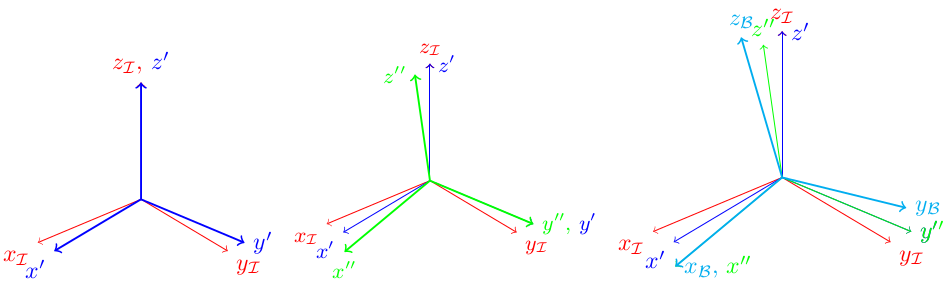
\includegraphics[width=0.9\textwidth]{images/euler.png}
\end{center}

有了欧拉角之后,给定一个旋转矩阵,我们可以按照公式\ref{eqn:euler}从旋转矩阵中求出三个欧拉角,更好地分析这个旋转矩阵的性质。另一方面,如果我们想构造一个旋转矩阵,就可以先设定三个想要的欧拉角,然后计算出所需的旋转矩阵。

另外,因为在机体坐标系中我们的三个轴有自己根据飞行器物理特性而定的名字,所以有时候我们也用三个轴来指代欧拉角。本节我们介绍的欧拉角也被叫做“yaw-pitch-roll”欧拉角,因为我们先在偏航轴进行旋转操作,然后是俯仰、最后是滚转。

\subsubsection{欧拉角与角速度}\label{sec:eulerandangular}
欧拉角的表示给我们提供了一种离散化旋转微分方程的思路,同时也可以让我们换一个思路理解角速度。让我们回顾旋转微分方程\ref{eqn:rdot},为了方便介绍,我们给方程中的旋转矩阵加上下标
$$
\dot{{\bf R}}_{eb} = {\bf R}_{eb}\lfloor \vv{\omega} \ \times \rfloor
$$
让我们先把这个方程摆在这里,然后用欧拉角和导数的定义重新推导一下这个方程。

当旋转矩阵${\bf R}_{eb}$随时间发生变化的时候,因为大地坐标系$e$始终静止,而机体坐标系$b$在运动,所以我们可以把每个时刻的机体坐标系$b$加上与时间相关的描述符。如果$t$时刻的旋转矩阵是${\bf R}_{eb(t)}$,则一个很短的时间段$\Delta t$之后的旋转矩阵则是${\bf R}_{eb(t+\Delta t)}$。根据旋转矩阵连续变换的原理,我们有
\begin{equation}\label{eqn:discreterot}
{\bf R}_{eb(t+\Delta t)} = {\bf R}_{eb(t)}{\bf R}_{b(t)b(t+\Delta t)}
\end{equation}

又根据导数的定义,我们可以把$\dot{{\bf R}}_{eb}$写成
$$
\dot{{\bf R}}_{eb(t)} = \lim_{\Delta t \to 0}\frac{1}{\Delta t}[{\bf R}_{eb(t+\Delta t)} - {\bf R}_{eb(t)}]
$$
根据前两个式子,我们能得到
$$
\dot{{\bf R}}_{eb(t)} = \lim_{\Delta t \to 0}\frac{{\bf R}_{eb(t)}}{\Delta t}[{\bf R}_{b(t)b(t+\Delta t}) - {\bf I}]
$$
现在我们关注${\bf R}_{b(t)b(t+\Delta t)}$的形式,它是一个旋转矩阵,所以肯定能用欧拉角来表示,我们把它写成
$$
{\bf R}_{b(t)b(t+\Delta t)} = {\bf R}_x(\Delta\phi){\bf R}_y(\Delta\theta){\bf R}_z(\Delta\psi)
$$
因为$\Delta t$是一个小量,则上述三个欧拉角也都是小量,对于小量角度,我们可以近似
$$
\cos\Delta\theta \approx 1 \ \ \ \ \ \sin\Delta\theta \approx \Delta\theta \ \ \ \ \ \Delta\theta\Delta\psi \approx 0
$$
这样公式\ref{eqn:euler}就可以简化为
$$
{\bf R}_{b(t)b(t+\Delta t)} =
\begin{bmatrix}
1 & -\Delta\psi & \Delta\theta\\
\Delta\psi & 1 & -\Delta\phi \\
-\Delta\theta & \Delta\phi & 1
\end{bmatrix} 
$$
在前面的角速度定义里我们介绍过$\omega_1$,$\omega_2$和$\omega_3$分别表示绕$x$,$y$和$z$轴的旋转,而从欧拉角的定义中我们看到$\Delta\phi$,$\Delta\theta$和$\Delta\psi$分别表示绕$x$,$y$和$z$轴的旋转角度,显然我们有
$$
\Delta\phi = \omega_1\Delta t
$$
$$
\Delta\theta = \omega_2\Delta t
$$
$$
\Delta\psi = \omega_3\Delta t
$$
所以我们可以得到
$$
{\bf R}_{b(t)b(t+\Delta t)} =
\begin{bmatrix}
1 & -\omega_3\Delta t & \omega_2\Delta t\\
\omega_3\Delta t & 1 & -\omega_1\Delta t \\
-\omega_2\Delta t & \omega_1\Delta t & 1
\end{bmatrix} 
= 
\begin{bmatrix}
0 & -\omega_3 & \omega_2\\
\omega_3 & 0 & -\omega_1 \\
-\omega_2 & \omega_1 & 0
\end{bmatrix}\Delta t + {\bf I} 
=
\lfloor \vv{\omega} \ \times \rfloor \Delta t + {\bf I} 
$$
我们又一次看到了角速度构成的反对称矩阵。在仔细思考这是一种巧合还是惊人的数学之美之前,让我们先继续完成推导。所以
$$
\dot{{\bf R}}_{eb(t)} = 
\lim_{\Delta t \to 0}\frac{{\bf R}_{eb(t)}}{\Delta t}[{\bf R}_{b(t)b(t+\Delta t)} - {\bf I}] 
=
\lim_{\Delta t \to 0}\frac{{\bf R}_{eb(t)}}{\Delta t}(\lfloor \vv{\omega} \ \times \rfloor \Delta t)
=
{\bf R}_{eb(t)}\lfloor \vv{\omega} \ \times \rfloor
$$
我们获得了公式\ref{eqn:rdot}。另外,通过公式\ref{eqn:discreterot}我们还得到了公式\ref{eqn:rdot}的一个离散化表示形式
\begin{equation}\label{eqn:discreterdot_euler}
{\bf R}_{eb(t+\Delta t)} = {\bf R}_{eb(t)}(\lfloor \vv{\omega} \ \times \rfloor \Delta t + {\bf I})
\end{equation}

本节的推导将欧拉角与之前介绍的旋转微分方程联系了起来。如果不通过欧拉角进行参数化,我们就很难把${\bf R}_{b(t)b(t+\Delta t)}$写成表达式进行分析。

更重要的是,公式\ref{eqn:discreterdot_euler}也给出了一个可以应用在工程实际上的方程。如果飞行器上安装着一个能够获取机体角速度的传感器,我们可以写一个程序实时更新飞行器的三个欧拉角。在程序的每一个循环里,我们把前一时刻的欧拉角拿到,构造旋转矩阵,然后根据公式\ref{eqn:discreterdot_euler}来编程,就能够通过角速度传感器的测量值获得这一时刻的旋转矩阵,最后我们从新的旋转矩阵提取出欧拉角,完成循环。有了这个程序之后,我们就实现了对飞行器的\textbf{姿态估计},这是多旋翼飞行器控制中的关键步骤。当然在实际中,由于角速度传感器固有的元器件缺陷,仅靠角速度传感器不能长时间准确地进行姿态估计,我们还需要其他的传感器进行辅助,本教程中就不再讨论其中的细节了。
\subsubsection{万向节死锁(Gimbal Lock)}
欧拉角虽然是一种直观的表示,使用也很方便,但它在数学上并不简洁完备。它可以看做是一种映射的关系:
\begin{align*}
 f: \ \ \ \ \mathbb{R}^3 & \rightarrow SO(3) \\
	[\psi, \theta, \phi] & \rightarrow {\bf R}	
\end{align*}
但是这个映射关系不是一种函数关系,可能有多组参数对应同一个旋转矩阵。欧拉角最大的问题是著名的万向节死锁(Gimbal Lock),这种情况下会有无穷多组参数对应同一个旋转矩阵。

我们回顾公式\ref{eqn:eulerparts}
$$
{\bf R}_{eb} = 
\begin{bmatrix}
1 & 0 & 0 \\
0 & \cos\phi & -\sin\phi \\
0 & \sin\phi & \cos\phi 
\end{bmatrix} 
\begin{bmatrix}
\cos\theta & 0 & \sin\theta\\
0 & 1 & 0\\
-\sin\theta & 0 & \cos\theta \\
\end{bmatrix}
\begin{bmatrix}
\cos\psi & - \sin\psi & 0\\
\sin\psi & \cos\psi & 0\\
0 & 0 & 1
\end{bmatrix}
$$
如果因为某些原因,$\theta$等于$90$度,则$\cos\theta = 0$,$\sin\theta = 1$。此时${\bf R}_{eb}$的表达式会变成
$$
{\bf R}_{eb} = 
\begin{bmatrix}
1 & 0 & 0 \\
0 & \cos\phi & -\sin\phi \\
0 & \sin\phi & \cos\phi 
\end{bmatrix} 
\begin{bmatrix}
0 & 0 & 1\\
0 & 1 & 0\\
-1 & 0 & 0 \\
\end{bmatrix}
\begin{bmatrix}
\cos\psi & - \sin\psi & 0\\
\sin\psi & \cos\psi & 0\\
0 & 0 & 1
\end{bmatrix}
$$
我们把三个矩阵乘起来,再利用三角函数的性质化简这个表达式,可以获得
$$
{\bf R}_{eb} = 
\begin{bmatrix}
0 & 0 & 1 \\
\sin(\phi + \psi) & \cos(\phi + \psi) & 0 \\
\cos(\phi + \psi) & \sin(\phi + \psi) & 0 
\end{bmatrix}
$$

上式作为一个旋转矩阵,$\phi$和$\psi$的地位是一样的。如果我们构造这样一个旋转矩阵,改变两者中任何一个的数值,结果都是绕同一个轴旋转的操作。这种情况下我们说旋转矩阵失去了一个自由度。考虑如下场景:一个飞机起飞之后,把俯仰角拉到了90度,如果飞机的控制器使用欧拉角来控制飞机,那么这时只能够控制飞行器的横滚,而不能控制偏航。万向节死锁在惯性导航、飞行器控制、计算机图形学等很多实际的工程项目中造成了问题,而且由于它是欧拉角固有的缺陷,所以只能用一些工程性比较强的办法来解决。

因为欧拉角有很多种不统一的旋转顺序标准,让新手学习时有很大的不便。再加上欧拉角有万向节死锁的问题,而且通过欧拉角做姿态控制无法得到一个理论上较为严格的控制律,所以在多旋翼的控制中,我们并不用欧拉角作为旋转矩阵参数化的方法,而是用四元数。

\subsection{四元数}
在二维平面上,复数可以用来建立复平面并表示复平面上的点。四元数则是拓展了复数的思路,用来表示三维空间中的点。William Rowan Hamilton创造性地引入了第四个维度,使四元数有了更多丰富的性质,可以用来表示旋转。我们定义一个四元数如下
$$
\bar{q} = q_4 + q_1\mathbf{i} + q_2\mathbf{j}+ q_3\mathbf{k}
$$  
上式中,$q_1$,$q_2$,$q_3$和$q_4$是四个标量,不同的资料里可以见到不同的表示符号,有些资料中将$q_4$表示为$q_0$,有些资料则用$x$,$y$,$z$和$w$表示这四个数值,读者需要注意他们的顺序和意义。

四元数的核心思想在于,用$1$,$\mathbf{i}$,$\mathbf{j}$和$\mathbf{k}$代表$\mathbb{R}^4$的一组基,每一个四元数都是这组基的线性组合。四元数的基满足如下关系
$$
\mathbf{i}^2 = \mathbf{j}^2 = \mathbf{k}^2 = \mathbf{i}\mathbf{j}\mathbf{k} = -1
$$
$$
\mathbf{i}\mathbf{j}=\mathbf{k}
$$
$$
\mathbf{j}\mathbf{k}=\mathbf{i}
$$
$$
\mathbf{k}\mathbf{i}=\mathbf{j}
$$
我们注意到上述定义中$\mathbf{i}\mathbf{j}=\mathbf{k}$。这里值得读者仔细注意。\textbf{四元数有两种定义,在Hamilton自己最早的定义中$\mathbf{i}\ \mathbf{j}=\mathbf{k}$。但是后来在NASA JPL开始使用四元数之后,他们在定义中采用了$\mathbf{i}\ \mathbf{j}=-\mathbf{k}$}。可能NASA吃了很多欧拉角的亏,所以在20世纪后期大力推广四元数作为旋转矩阵的参数化方式。四元数近年来广受欢迎主要得益于NASA的推广,因此网上的很多资料中都按照NASA的定义采用了左手坐标系,即使他们依然用四元数旋转右手坐标系。两种定义在最初的表达式中差别极小,但是会给后续很多公式的推导造成细微又迷惑的区别。很多人在查找四元数的相关资料时,会在不同的资料中看到同一个公式在不同的资料里恰巧差了一些正负号的尴尬情况。因此读者对于$\mathbf{i}$和$\mathbf{j}$相乘的结果要格外小心,最好能够自己选定。\textbf{本篇教程中的四元数采用Hamilton的古典定义},如果读者对网上的资料有疑问,可以到爱尔兰都柏林的Brougham桥上看看,Hamilton把他关于四元数的发现:$\mathbf{i}^2 = \mathbf{j}^2 = \mathbf{k}^2 = \mathbf{i}\mathbf{j}\mathbf{k} = -1$刻在了桥头。

有时我们也称$q_4$是$\bar{q}$的标量部分,$\vv{q} = [q_1 \ \ q_2 \ \ q_3]^T$是$\bar{q}$的矢量部分,并且把四元数表示成如下的形式
$$
\bar{q} 
=
				   \begin{bmatrix}
                      q_1\\
                      q_2\\
                      q_3\\
                      q_4
                   \end{bmatrix}
              =  \begin{bmatrix}
                      \vv{q}\\
                      q_4
                   \end{bmatrix} 
$$

特别地,如果四元数的四个数满足下列关系
\begin{equation}\label{equ:quad_theta}
      \mathbf{q} = 
      \begin{bmatrix}
        q_1\\
        q_2\\
        q_3\\
      \end{bmatrix} =
      \begin{bmatrix}
        k_x sin(\theta/2)\\
        k_y sin(\theta/2)\\
        k_z sin(\theta/2)\\
      \end{bmatrix} =  \vv{k} sin(\theta/2),
      \ \ \ \ \ 
      q_4 = cos(\theta/2)
\end{equation}
其中$\vv{k} = [k_x \ \ \ k_y \ \ \ k_z]^T$是一个单位向量($\| \vv{k}\| = 1$),所以也可以明显看出
$$
q_1^2+q_2^2+q_3^2+q_4^2 = 1
$$
满足这种关系的四元数叫做\textbf{旋转四元数}。读者可以看出实际上$\vv{k}$是一个旋转轴,而$\theta$是一个绕轴旋转的角度。因此旋转四元数与旋转矩阵有非常直接的对应关系,可以用来表示旋转变换。它也是一种和旋转矩阵的映射关系
\begin{align*}
 f: \ \ \ \ \mathbb{R}^4 & \rightarrow SO(3) \\
	[q_1 \ \ q_2 \ \ q_3 \ \ q_4] & \rightarrow {\bf R}	
\end{align*}
相比起欧拉角来说,旋转四元数的数学特性好了很多,它和旋转矩阵的映射是二对一的关系。读者稍加思考就能想到,在定义\ref{equ:quad_theta}中,“绕$\vv{k}$轴旋转$\theta$度角”等价于绕$-\vv{k}$轴旋转$-\theta$度角。关于这一点我们不再深入探讨,读者可以自己查阅相关资料。

在本节剩余的部分里,如果没有另外说明,我们讨论的所有四元数都是旋转四元数。

如果说旋转四元数能够用来实现旋转变换,那么它应该也能够写成类似
$$
p_e = {\bf R}_{eb}p_b
$$
这样的形式,而且也能像旋转矩阵那样连续进行变换
$$
{\bf R}_{eb} = {\bf R}_{ea}{\bf R}_{ab}
$$

我们确实可以写出
$$
\bar{q}_{eb} = \bar{q}_{ea}\bar{q}_{ab}
$$
这样的形式,不过这里的乘法不是矩阵乘法,而是四元数特别的乘法。而用四元数来变换三维矢量,也需要借助涉及四元数乘法的一个特殊的操作。下面我们将会逐步进行介绍。

首先我们介绍四元数的乘法。假设我们有两个四元数$\bar{p}$和$\bar{q}$,我们定义它们相乘的结果如下
\begin{align}
\bar{q} \otimes \bar{p} = &  (q_4 + q_1\mathbf{i} + q_2\mathbf{j}+ q_3\mathbf{k}) (p_4 + p_1\mathbf{i} + p_2\mathbf{j}+ p_3\mathbf{k})   \\
 = & q_4 p_4 - q_1 p_1 - q_2 p_2 - q_3 p_3 + (q_4 p_1 + q_1 p_4 - q_2 p_3 + q_3 p_2 ) \mathbf{i}\\
                 = &\begin{bmatrix}
                      q_4 & -q_3 & q_2 & q_1 \\
                      q_3 & q_4 & -q_1 & q_2 \\
                      -q_2 & q_1 & q_4 & q_3 \\
                      -q_1 & -q_2 & -q_3 & q_4 \\
                     \end{bmatrix} \begin{bmatrix}
                      p_1\\p_2\\p_3\\p_4
                     \end{bmatrix} \\
\label{eqn:quatmultimtx}          = & \begin{bmatrix}
                      q_4\mathbf{I}_3+\lfloor \vv{q} \ \times \rfloor   & \vv{q} \\
                      -\vv{q}^T & q_4  
                     \end{bmatrix} \begin{bmatrix}
                                     \vv{p}\\
                                     p_4
                                \end{bmatrix} =  \begin{bmatrix}
                                            p_4\mathbf{I}_3-\lfloor \vv{p} \ \times \rfloor   & \vv{p} \\
                                            -\vv{p}^T & p_4  
                                    \end{bmatrix} \begin{bmatrix}
                                            \vv{q}\\
                                            q_4
                                    \end{bmatrix}
\end{align}
注意到公式\ref{eqn:quatmultimtx}中我们可以把四元数的乘法$\otimes$用普通的矩阵和四维向量的乘法来表示。这也说明了四元数的乘法是不可交换的,$\bar{q} \otimes \bar{p} \neq \bar{p} \otimes \bar{q}$。

通过乘法的定义易证得,任何一个四元数与
$$
\bar{q}_I = 
\begin{bmatrix}
0 \\ 0 \\ 0 \\ 1
\end{bmatrix}
$$
相乘,结果都是这个四元数本身。所以我们把$\bar{q}_I$叫做单位四元数,与旋转矩阵中的单位矩阵$\mathbf{I}$对应。

四元数与旋转矩阵同样具有逆运算,给定一个四元数$\bar{q}$,我们可以证明
$$
\bar{q}^{-1} = 
\begin{bmatrix}
                      -\vv{q}\\
                      q_4
\end{bmatrix}
$$
是它的逆运算,也就是说
$$
\bar{q}^{-1} \otimes \bar{q} = \bar{q} \otimes \bar{q}^{-1} = \bar{q}_I
$$
对四元数求逆之后得到的这个四元数也被称为共轭四元数(conjugate quaternion),这个名字是由共轭复数推广而来的。

现在我们定义用四元数旋转一个三维矢量的方式。我们继续用之前已经熟悉的坐标系$e$和坐标系$b$之间的变换为例子,假设我们已经知道这两个坐标系之间的旋转四元数是$\bar{q}_{eb}$,我们暂时可以先不关注这个四元数是通过什么方式获得的,我们就把它当做已知数写成$[q_1 \ \ q_2 \ \ q_3 \ \ q_4]^T$。为了旋转表示在坐标系$b$中的质点$\vv{p}_b$,我们首先构造一个标量部为零的四元数
$$
\bar{p}_b =  
\begin{bmatrix}
                      \vv{p}_b\\
                      0
\end{bmatrix}
$$
则根据四元数乘法计算下列表达式
\begin{equation}\label{eqn:quatrotexp}
\bar{p}_e =  
\begin{bmatrix}
                      \vv{p}_e\\
                      0
\end{bmatrix} = 
\bar{q}_{eb} \otimes \bar{p}_b \otimes \bar{q}^{-1}_{eb}
\end{equation}
得到的四元数$\bar{p}_e$中的矢量部分$\vv{p}_e$就是我们想要知道的质点在坐标系$e$中的表示。

人们获得这个定义的证明的历史已经不可考证,有可能是通过构造证明获得的,因为直接展开表达式可以证明上述定义与角轴法中的罗德里格斯公式(Rodrigues' rotation formula)有很大联系。在本篇教程中,我们不用深究这个这个定义的来源,把它当做一个已知的公式使用就好。

我们扔掉下标,借助四元数乘法的定义展开表达式\ref{eqn:quatrotexp},从中我们将可以看到四元数和旋转矩阵之间有趣的联系
\begin{align*}
\bar{q} \otimes \bar{p} \otimes \bar{q}^{-1} 
= & 
\begin{bmatrix}
q_4\mathbf{I}_3+\lfloor \vv{q} \ \times \rfloor   & \vv{q} \\
-\vv{q}^T & q_4  
\end{bmatrix} 
\begin{bmatrix}
\vv{p}\\
0
\end{bmatrix}\otimes \bar{q}^{-1}
\\
= &
%\begin{bmatrix}
%\end{bmatrix}
\begin{bmatrix}
q_4\vv{p} + \vv{q}\times\vv{p} \\
-\vv{q}^T\vv{p}
\end{bmatrix}
\otimes
\begin{bmatrix}
-\vv{q}\\
q_4
\end{bmatrix}
%\text{(把$\otimes$展开)}
\\
= &
\begin{bmatrix}
-\vv{q}^T\vv{p}{\bf I}_3 + \lfloor q_4\vv{p}+(\vv{q}\times\vv{p}) \ \times \rfloor &
q_4\vv{p} + \vv{q}\times\vv{p} \\
-(q_4\vv{p}+\vv{q}\times\vv{p})^T &
-\vv{q}^T\vv{p}
\end{bmatrix}
\begin{bmatrix}
-\vv{q}\\
q_4
\end{bmatrix}
\\
= &
\begin{bmatrix}
\vv{q}(\vv{q}^T\vv{p}) - q_4\vv{p}\times\vv{q} - \vv{q}\times\vv{p}\times\vv{q}+q_4^2\vv{p}+q_4\vv{q}\times\vv{p}\\
q_4\vv{q}^T\vv{p}+(\vv{q}\times\vv{p})^T\vv{q}-q_4\vv{q}^T\vv{p}
\end{bmatrix}
\end{align*}
上式中有两项需要特别注意。第一,根据叉乘的性质,$(\vv{q}\times\vv{p})^T\vv{q} = 0$,因此矩阵的整个第二行都等于零;第二,我们把$\vv{q}\times\vv{p}\times\vv{q}$单独展开并化简可以获得
\begin{equation}\label{eqn:crosscross}
\vv{q}\times\vv{p}\times\vv{q} = 
\begin{bmatrix}
q_2^2+q_3^2	&	-q_1q_2		&	-q_1q_3	\\
-q_1q_2		&	q_1^2+q_3^2	&	-q_2q_3	\\
-q_1q_3		&	-q_2q_3		&	q_1^2+q_2^2
\end{bmatrix}\vv{p}
\end{equation}
又因为
$$
\vv{q}\vv{q}^T = 
\begin{bmatrix}
q_1^2	&	q_1q_2		&	q_1q_3	\\
q_1q_2		&	q_2^2	&	q_2q_3	\\
q_1q_3		&	q_2q_3	&	q_3^2
\end{bmatrix}
$$
再加上$q_1^2+q_2^2+q_3^2+q_4^2 = 1$的性质,所以
$$
\vv{q}\times\vv{p}\times\vv{q} = ((1-q_4^2){\bf I} - \vv{q}\vv{q}^T)\vv{p}
$$
我们继续对乘法表达式的化简
\begin{align*}
\bar{q} \otimes \bar{p} \otimes \bar{q}^{-1} 
= & 
\begin{bmatrix}
\vv{q}(\vv{q}^T\vv{p}) - q_4\vv{p}\times\vv{q} - ((1-q_4^2){\bf I} - \vv{q}\vv{q}^T)\vv{p} + q_4^2\vv{p}+q_4\vv{q}\times\vv{p} \\
0  
\end{bmatrix} 
\\
= &
\begin{bmatrix}
(2q_4^2-1)\vv{p} + 2q_4\lfloor \vv{q} \ \times \rfloor \vv{p}  + 2\vv{q}\vv{q}^T\vv{p} \\
0  
\end{bmatrix} 
\\
= &
\begin{bmatrix}
(2q_4^2-1) + 2q_4\lfloor \vv{q} \ \times \rfloor   + 2\vv{q}\vv{q}^T & {\bf 0}_{3x1}\\
{\bf 0}_{1x3}  & 0
\end{bmatrix}\vv{p}
\end{align*}
推导到这里,我们可以发现
$$
\vv{p}_e = [(2q_4^2-1) + 2q_4\lfloor \vv{q} \ \times \rfloor   + 2\vv{q}\vv{q}^T]\vv{p}_b
$$
我们获得了矩阵${\bf R}_{eb}$和四元数$\bar{q}_{eb}$的关系,
$$
{\bf R}_{eb} = (2q_4^2-1) + 2q_4\lfloor \vv{q} \ \times \rfloor   + 2\vv{q}\vv{q}^T
$$
现在我们可以使用表达式\ref{eqn:quatrotexp}去旋转向量了。
%\begin{bmatrix}
%\end{bmatrix}
根据四元数旋转向量的表达式,我们也能看出四元数乘法和连续旋转变换的关系
$$
\bar{p}_a = \bar{q}_{ab} \otimes \bar{p}_b \otimes \bar{q}^{-1}_{ab}
$$
\begin{align*}
\bar{p}_e = & \ \ \bar{q}_{ea} \otimes \bar{p}_a \otimes \bar{q}^{-1}_{ea}\\
		  = & \ \ \bar{q}_{ea} \otimes \bar{q}_{ab} \otimes \bar{p}_b \otimes \bar{q}^{-1}_{ab} \otimes \bar{q}^{-1}_{ea}\\
		  = & \ \ \bar{q}_{eb} \otimes \bar{p}_b \otimes \bar{q}^{-1}_{eb}
\end{align*}
\subsubsection{四元数与角速度}
四元数能够像欧拉角那样,帮助我们进行旋转微分方程的离散化。在本小节中,我们把章节\ref{sec:eulerandangular}所做的推导再重新用四元数推导一次,这可以帮助我们更好地理解四元数。

首先我们把章节\ref{sec:eulerandangular}中的一些公式再摆出来
\begin{equation*}
{\bf R}_{eb(t+\Delta t)} = {\bf R}_{eb(t)}{\bf R}_{b(t)b(t+\Delta t)}
\end{equation*}
$$
\dot{{\bf R}}_{eb(t)} = \lim_{\Delta t \to 0}\frac{1}{\Delta t}[{\bf R}_{eb(t+\Delta t)} - {\bf R}_{eb(t)}]
$$

根据前面介绍的四元数的特性,我们可以确信同样的表达式对四元数来说也是成立的
\begin{equation*}
\bar{q}_{eb(t+\Delta t)} = \bar{q}_{eb(t)}\bar{q}_{b(t)b(t+\Delta t)}
\end{equation*}
$$
\dot{\bar{q}}_{eb(t)} = \lim_{\Delta t \to 0}\frac{\bar{q}_{eb(t)}}{\Delta t}[\bar{q}_{b(t)b(t+\Delta t)} - \bar{q}_I]
$$
我们这里默认四元数之间的操作是四元数乘法,而不是普通乘法。

和欧拉角相比,用四元数表示微小的旋转$\bar{q}_{b(t)b(t+\Delta t)}$比较直接。从定义\ref{equ:quad_theta}可以看出,如果$\theta$是一个很小的角度$\Delta \theta$,则对应的小旋转就是
$$
\bar{q}_{b(t)b(t+\Delta t)} =
	\begin{bmatrix} 
        k_x \Delta\theta/2\\
        k_y \Delta\theta/2\\
        k_z \Delta\theta/2\\
      	1
	\end{bmatrix}
$$
我们发现
$$
\frac{\bar{q}_{b(t)b(t+\Delta t)} - \bar{q}_I}{\Delta t} =
	\begin{bmatrix} 
        \frac{1}{2}k_x \frac{\Delta\theta}{\Delta t}\\
        \frac{1}{2}k_y \frac{\Delta\theta}{\Delta t}\\
        \frac{1}{2}k_z \frac{\Delta\theta}{\Delta t}\\
      	0
	\end{bmatrix}
$$
这恰好是公式\ref{eqn:omegadef}中给出的角速度定义乘以$\frac{1}{2}$,因此
$$
\dot{\bar{q}}_{eb(t)} = \frac{1}{2}\bar{q}_{eb(t)}\otimes
	\begin{bmatrix} 
        \omega_1\\ 
        \omega_2\\ 
        \omega_3\\
      	0
	\end{bmatrix} = 
	\frac{1}{2}\bar{q}_{eb(t)}
	\begin{bmatrix} 
        \vv{\omega}\\
      	0
	\end{bmatrix}
$$

同样地,一个基于四元数的离散化的旋转微分方程也可以由上述推导获得
\begin{equation}\label{eqn:discreterdot_quat}
\bar{q}_{eb(t+\Delta t)} = \bar{q}_{eb(t)}(
	\frac{1}{2}	
	\begin{bmatrix} 
        \vv{\omega}\\
      	0
	\end{bmatrix}\Delta t + q_I
	)
\end{equation}

同公式\ref{eqn:discreterdot_euler}一样,公式\ref{eqn:discreterdot_quat}也可以用做飞行器的姿态估计。另外,基于四元数的姿态控制算法也被证明有着更好的理论稳定性,以及数值稳定性。读者可以阅读我和同事合作的论文\cite{7139416}看到一种基于四元数的姿态控制算法的实现方式。另一篇更为早期的文章\cite{5717652}给出了同样的结果,但是使用了不同的证明思路。
\ \\
\ \\
\ \\
本章中我们介绍了两种参数化旋转矩阵的方式,并介绍了两种方式下推导旋转微分方程的过程。建议读者自己通过笔和纸将本章中的推导重新演算一遍,并做一份四元数或者欧拉角的参考表格以备使用时查找。

本章中并未介绍欧拉角和四元数之间的转换,读者可根据欧拉角与旋转矩阵的关系、四元数与旋转矩阵的关系自行推导欧拉角和四元数之间的转换公式。

\section{欧拉方程}\label{sec:euler}
​根据牛顿第二定律,对于刚体的位置$p(t)$、速度$\dot{p}(t)$、加速度$\ddot{p}(t)$来说,给定外力$F(t)$和初始状态$p(0)$和$\dot{p}(0)$以后,系统的状态是由如下的二阶常微分方程确定的:
\begin{equation}\label{eqn:newton2}
\ddot{p}(t) = \frac{F(t)}{m}
\end{equation}
其中$m$是刚体的质量。

对应地,对于绕定轴旋转的刚体的角度、角速度和角加速度来说,则是欧拉方程决定了系统的状态,它同样也是二阶常微分方程。相比于牛顿第二定律来说,由于旋转导致了坐标系不断变化,因此在方程中需要考虑角速度对系统的状态的影响。我们先不加说明地给出欧拉方程如下:
\begin{equation}
\vv{M} = {\bf I}\dot{\vv{\omega}} + \vv{\omega} \times {\bf I}\vv{\omega}
\end{equation}


本章将介绍角动量和惯性张量,并结合角速度的特性推导欧拉方程。本章内容和章节\ref{sec:rotmtx}以及\ref{sec:angular}联系较为紧密,因为理解欧拉方程的关键在于理解角速度以及旋转坐标系对物理量的影响。
\subsection{质点角动量}
绕定轴旋转的质点,距离旋转轴为$\vv{r}$,施加在质点力为$F$,则质点相对于定轴的力矩为

\begin{center}
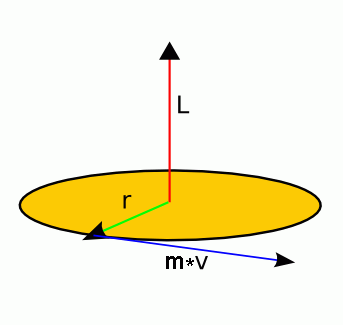
\includegraphics[width=0.6\textwidth]{images/angularmomentum.png}
\end{center}

$$
\vv{M} = \vv{r} \times \vv{F}
$$

因为
$$
\vv{F} = m \vv{a} = m \frac{d\vv{v}}{dt}
$$
则
$$
\vv{M} = \vv{r} \times m \frac{d\vv{v}}{dt}
$$

如果我们定义角动量
$$
\vv{L} = \vv{r} \times m \vv{v}
$$
则可以看到力矩是角动量的微分
$$
\frac{d\vv{L}}{dt} = \frac{d(\vv{r} \times m \vv{v})}{dt} = \frac{d\vv{r}}{dt} \times m \vv{v} + \vv{r}\times m\frac{d\vv{v}}{dt} = \vv{M}
$$
其中
$
\frac{d\vv{r}}{dt} \times m \vv{v} = \vv{v} \times m \vv{v} = \vv{0} 
$
\subsection{刚体角动量和惯性张量}
对于绕定轴旋转的刚体来说,我们可以把它看成一个大量质点构成的集合,所以它的角动量可以被看成是它的所有质点的角动量的集合。对于它的每一个小的质量单元,我们把角动量写成
$$
\Delta \vv{L} = \vv{r} \times \Delta m(\vv{r}) \vv{v}(\vv{r})
$$
这里的$\Delta m(\vv{r})$代表$\Delta m$是关于$\vv{r}$的函数。而对于整个刚体,我们可以把所有的质量单元积分起来获得刚体的角动量,我们把离散的小量符号$\Delta$换成微分符号$d$
$$
\vv{L} = \int d\vv{L} = \int \vv{r} \times dm(\vv{r}) \vv{v}(\vv{r})
$$
在章节\label{sec:angular}中,我们用不同方法推导出了速度和角速度的关系。把$\vv{v} = \vv{\omega}\times\vv{r}$带入表达式,我们得到
\begin{equation}
\vv{L} = \int \vv{r} \times \vv{\omega}\times\vv{r} dm(\vv{r})
\end{equation}
在前一章中我们推导过三个向量连续叉乘的结果为表达式\ref{eqn:crosscross},这里相似地我们可以展开$\vv{r} \times \vv{\omega}\times\vv{r}$,获得
$$
\vv{r} \times \vv{\omega}\times\vv{r} = 
\begin{bmatrix}
y^2+z^2	&	-xy		&	-xz	\\
-xy		&	x^2+z^2	&	-yz	\\
-xz		&	-yz		&	x^2+y^2
\end{bmatrix}\vv{\omega}
$$
其中$\vv{r} = [x \ \ y \ \ z]^T$。把展开后的表达式带入上式,我们可以得到
\begin{equation}\label{eqn:momemtum}
\vv{L} = 
\begin{bmatrix}
\int (y^2+z^2) dm	&	-\int xy dm		&	-\int xz dm	\\
-\int xy dm		&	\int (x^2+z^2) dm	&	-\int yz dm	\\
-\int xz dm		&	-\int yz dm		&	\int (x^2+y^2) dm
\end{bmatrix}\vv{\omega}
\end{equation}
公式\ref{eqn:momemtum}中的矩阵形式的项叫做惯性张量(Inertia Tensor)。它像质量$m$一样,描述了刚体在旋转上的特性。我们通常将他记为一个特殊的符号
$$
{\bf I} = 
\begin{bmatrix}
\int (y^2+z^2) dm	&	-\int xy dm		&	-\int xz dm	\\
-\int xy dm		&	\int (x^2+z^2) dm	&	-\int yz dm	\\
-\int xz dm		&	-\int yz dm		&	\int (x^2+y^2) dm
\end{bmatrix}
$$
这样角动量就写成了
$$
\vv{L} = {\bf I}\vv{\omega}
$$
与动量
$$
\vv{p} = m\vv{v}
$$
颇为对应。

\subsection{推导欧拉方程}
对于飞行器控制来说,我们关注的是,给飞行器施加一个力矩,飞行器的角速度会如何变化。所以我们需要建立力矩和飞行器角速度的关系,因此要对$\vv{L}$的表达式求导
$$
\frac{d\vv{L}}{dt} = \dot{{\bf I}}\omega + {\bf I} \dot{\vv{\omega}}   
$$
表达式中最麻烦的是$\dot{{\bf I}}$的形式应该是什么。为了推导惯性张量的微分,我们换一种形式来表达角动量。

常用的一个缩写形式是
$$
I_{xx} = \int (y^2+z^2) dm
$$
$$
I_{xy} = \int xy dm
$$
据此,我们进一步把公式\ref{eqn:momemtum}展开,获得
$$
\vv{L} = 
\begin{bmatrix}
I_{xx}\omega_x-I_{xy}\omega_y-I_{xz}\omega_z\\
-I_{yx}\omega_x+I_{yy}\omega_y-I_{yz}\omega_z\\
-I_{zx}\omega_x-I_{zy}\omega_y+I_{zz}\omega_z
\end{bmatrix}
$$

在章节\ref{sec:movingcor}中,我们提到旋转坐标系对坐标系中物理量的影响。对角动量来说,刚体在转动时,它的机体坐标系在不断变化,影响了$\vv{r}_e$的表示,进而也影响了与$\vv{r}_e$直接相关的惯性张量的表示。我们采用和章节\ref{sec:movingcor}类似的推导方法,先把角动量写成
\begin{align*}
\vv{L} = & \ L_x \vv{i} + L_y \vv{j} + L_z \vv{k} \\
	   = & \ (I_{xx}\omega_x-I_{xy}\omega_y-I_{xz}\omega_z)\vv{i} + \\
	   = & \ (-I_{yx}\omega_x+I_{yy}\omega_y-I_{yz}\omega_z)\vv{j} + \\
	   = & \ (-I_{zx}\omega_x-I_{zy}\omega_y+I_{zz}\omega_z)\vv{k} 
\end{align*}

这样$\vv{L}$的导数为
$$
\frac{d\vv{L}}{dt} =  \dot{L}_x \vv{i} + \dot{L}_y \vv{j} + \dot{L}_z \vv{k} + L_x \dot{\vv{i}} + L_y \dot{\vv{j}} + L_z \dot{\vv{k}} 
$$

在章节\ref{sec:movingcor}中我们已经解释过,这样求导可以把物理量的时间变化和坐标系旋转导致的变化之间的影响分解开来。在$L_x$,$L_y$和$L_z$中,和时间相关的量只有角速度$\vv{\omega}$,所以$\dot{L}_x = I_{xx}\dot{\omega}_x-I_{xy}\dot{\omega}_y-I_{xz}\dot{\omega}_z$,而我们早已证明了$\dot{\vv{i}} = \vv{\omega} \times \vv{i}$,因此经过一番不复杂的变换,我们可以获得
$$
\frac{d\vv{L}}{dt} = {\bf I}\dot{\vv{\omega}} + \vv{\omega}\times{\bf I}\vv{\omega}
$$

这也就是我们在章节开始给出的欧拉方程
$$
\vv{M} = {\bf I}\dot{\vv{\omega}} + \vv{\omega} \times {\bf I}\vv{\omega}
$$

\subsection{欧拉方程与多旋翼飞行器}
在多旋翼飞行器的控制中,欧拉方程和旋转微分方程是最核心的公式,我们把两个方程列出来如下
$$
\dot{{\bf R}} = {\bf R}\lfloor \vv{\omega} \ \times \rfloor
$$
$$
\vv{M} = {\bf I}\dot{\vv{\omega}} + \vv{\omega} \times {\bf I}\vv{\omega}
$$

在最基本的多旋翼飞行器控制器中,飞行器通过改变电机转速控制好三个轴的力矩,然后通过力矩和欧拉方程包含的二阶微分方程控制角速度,进而控制姿态角。多旋翼飞行器在空中飞行的时候,通过调整自己的姿态角来产生往某个方向的推力。所以系统位置微分方程\ref{eqn:newton2}中,F的x、y分量实际上是由姿态角决定的。

当然工程实践中,还有很多其他的问题需要考虑。为了飞行器能够在空中实现姿态稳定,还需要能够处理角速度信号、解算姿态角、计算电机转速和三轴力矩之间的关系、设计姿态控制器。这些问题超出了本教程的讨论范围。在此我们只指出一个需要注意的工程问题,以加深读者对欧拉方程和惯性张量的理解。

在很多四旋翼飞行器的控制当中,惯性张量
$$
{\bf I} = 
\begin{bmatrix}
\int (y^2+z^2) dm	&	-\int xy dm		&	-\int xz dm	\\
-\int xy dm		&	\int (x^2+z^2) dm	&	-\int yz dm	\\
-\int xz dm		&	-\int yz dm		&	\int (x^2+y^2) dm
\end{bmatrix}
$$
都会简化成
$$
{\bf I} = 
\begin{bmatrix}
\int (y^2+z^2) dm	&	0		&	0	\\
0		&	\int (x^2+z^2) dm	&	0	\\
0		&	0		&	\int (x^2+y^2) dm
\end{bmatrix}
$$
对于大部分四旋翼飞行器来说,因为飞行器有比较好的对称性,所以惯性张量中的很多项都会互相抵消。比如下图中两个电机,一个位置是$(x,y)$,另一个是$(x,-y)$,这样他们在积分项$\int xy dm$当中的和为0。然而对于很多异形的飞行器比如Inspire 1,或者机体下方悬挂着很重设备的飞行器,惯性张量中的项就很难被省略了。
%%%%%%%%%%%%%插个图
%%%%%%%%%%%%%

理论上,忽略不该忽略的惯性张量元素会导致飞行控制器的延迟增大,有些延迟无法被其他方式补偿掉。因此基于模型的控制器必须要获得比较精确的惯性张量,而不基于模型的控制器,如果要优化控制器的表现,依然需要仔细设定惯性张量。

\subsection{欧拉方程与机械陀螺}\label{sec:eulereqngyro}
在章节\ref{sec:angularsensor}中我们简单介绍了机械陀螺的原理。现在我们借助欧拉方程定量地去分析陀螺旋转时的特性。首先我们定义

因此在下图的机械陀螺的示例中,我们在input axis上施加一个力矩,output axis会开始转动。机械陀螺就是靠检测并抵抗output axis的转动来实现对input axis的力矩的测量的。

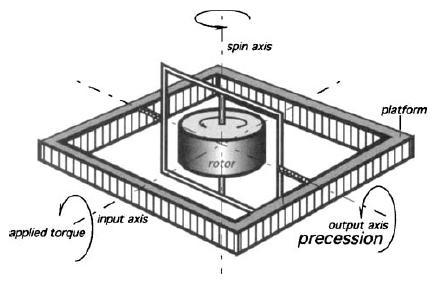
\includegraphics[width=0.8\textwidth]{images/gyroscopeAxes.jpg}

\section{通过仿真程序理解前述的知识}

在\url{https://github.com/paulyang1990/toy_code/tree/master/toy_ros_space/src/sim_drone}中有一个简单的四旋翼飞行器模拟器。在rigidBody.cpp中我们展示了如何通过程序实现欧拉方程的仿真。

\begin{center}
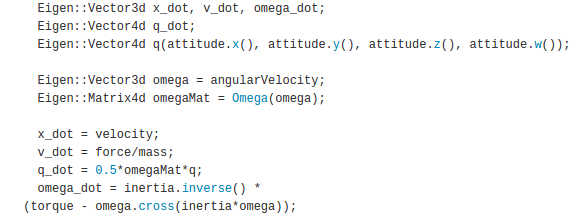
\includegraphics[width=0.9\textwidth]{images/code.png}
\end{center}

读者可以利用rigidBody.cpp和相关的辅助代码自行通过仿真程序理解欧拉方程。
\bibliographystyle{plain}
\bibliography{tutorial}
\end{document}
